\section{XMButton\-List  Class Reference}
\label{classXMButtonList}\index{XMButtonList@{XMButton\-List}}
{\tt \#include $<$XMWlist.h$>$}

Inheritance diagram for XMButton\-List::\begin{figure}[H]
\begin{center}
\leavevmode
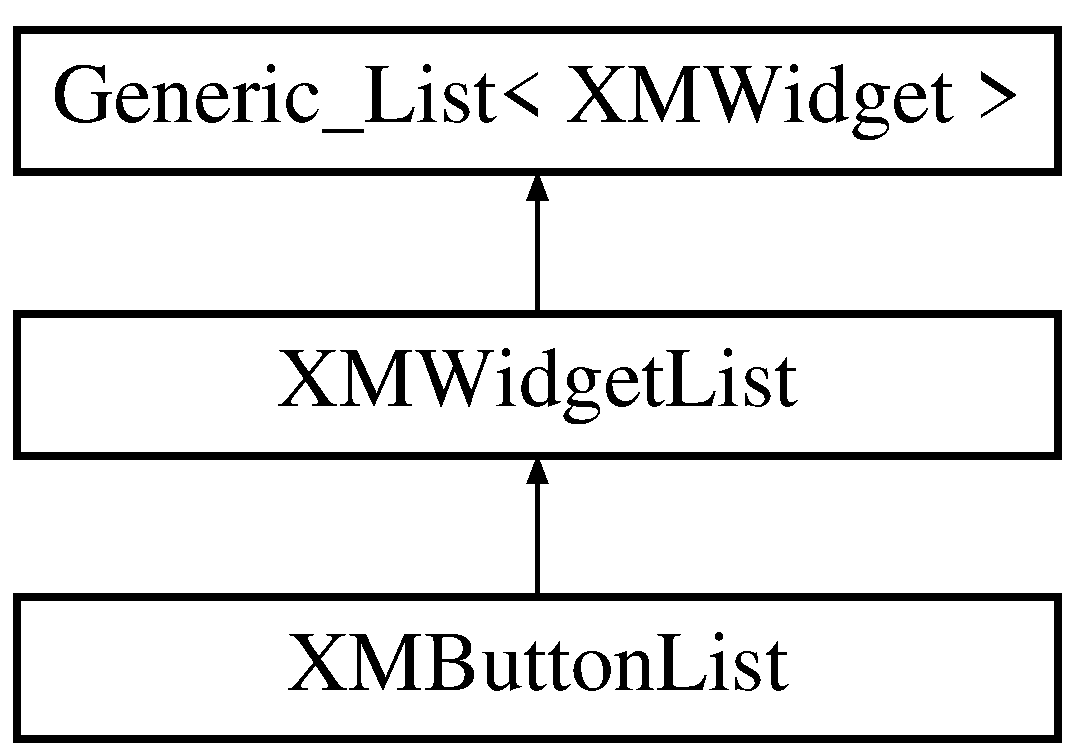
\includegraphics[height=3cm]{classXMButtonList}
\end{center}
\end{figure}
\subsection*{Public Methods}
\begin{CompactItemize}
\item 
void {\bf Enable} ()
\item 
void {\bf Disable} ()
\end{CompactItemize}


\subsection{Member Function Documentation}
\index{XMButtonList@{XMButton\-List}!Disable@{Disable}}
\index{Disable@{Disable}!XMButtonList@{XMButton\-List}}
\subsubsection{\setlength{\rightskip}{0pt plus 5cm}void XMButton\-List::Disable ()\hspace{0.3cm}{\tt  [inline]}}\label{classXMButtonList_a1}




Definition at line 385 of file XMWlist.h.

References XMWidget\-List::Set\-Attribute().\index{XMButtonList@{XMButton\-List}!Enable@{Enable}}
\index{Enable@{Enable}!XMButtonList@{XMButton\-List}}
\subsubsection{\setlength{\rightskip}{0pt plus 5cm}void XMButton\-List::Enable ()\hspace{0.3cm}{\tt  [inline]}}\label{classXMButtonList_a0}




Definition at line 382 of file XMWlist.h.

References XMWidget\-List::Set\-Attribute().

The documentation for this class was generated from the following file:\begin{CompactItemize}
\item 
{\bf XMWlist.h}\end{CompactItemize}
